\chapter{Introduction}
A \textit{web crawler} is a long running program that collects pages from the web and stores them to the
disk either in raw format or after extracting its contents. Sometimes they are also referred as
\textit{random walker}, \textit{worm}, \textit{spiders}, \textit{robot}. Crawlers serve variety of
purposes. Web search engines are very well-known systems powered internally through crawlers.
Other uses are web data mining for performing analytics, archiving portions of the web - a
relevant active project is the Wayback Machine from The Internet Archive\cite{netarchive} operating since 2000. Most recently,
there is an ongoing attempt from Software Heritage\cite{swheritage} that continuously crawl \& archive publicly available source code repositories on the web.
\\
\\
This thesis is an attempt to implement a small-scale, special purpose crawler for collecting data about
various job postings from a chosen set of job portals active on the web. As far as the scope of this thesis
is concerned, the work done here does not dive into cleaning \& analyzing the data set but instead focuses on its system design, implementation, and deployment of web crawler to perform data collection on given seed set. The crawler architecture builds on a open blueprint design of \textit{Mercator}\cite{mercator} which describes the design in enough detail but leaves out implementation specifics to developers.

\pagebreak

\section{Contributions}
\begin{itemize}
  \item \textbf{Use of Message Queue:} In one case, the paper doesn't provides information on how the subsystems that make up a crawler are connected together. This thesis makes use of message broker to facilitate collaboration between components thus providing asynchronous, event-driven style of communication. It also highlights its strengths \& weakness.
   \item \textbf{Crawl Ordering Problem:} A more crucial issue is without having a target to crawl, the problem of crawling becomes endless, infinite crawling even for specialized crawler such as this. This thesis discusses the crawl ordering strategy to shape its crawling only to specific content.
   \item \textbf{Distributing the crawl:} Furthermore, this thesis shows the shortcomings of linear hashing used for partitioning hosts to distribute the crawl and instead employs consistent hashing\cite{consisthash} algorithm and discuss its merits over it.
    \item \textbf{Development strategy:}  Given this complex program at hand, it becomes obvious to separate the concerns by developing and testing each component in isolated pieces. This thesis leverages docker containers to build the project in stages. It allows to split the development and production environment by building images for the target platform to run the component.
    \item \textbf{AWS Services:} For running the crawler activity, this thesis makes the most of AWS 12-month free tier access by combining together suite of services and sketches an infrastructure to setup, deploy and demonstrate the program.
    \item \textbf{Microservices:} Lastly, this thesis explains the philosophy, principles behind microservices \cite{microservices} by relating it to work done in this thesis.
\end{itemize}

\pagebreak

\section{Motivation}\index{Motivation}

\begin{figure}[h!]
  \centering
  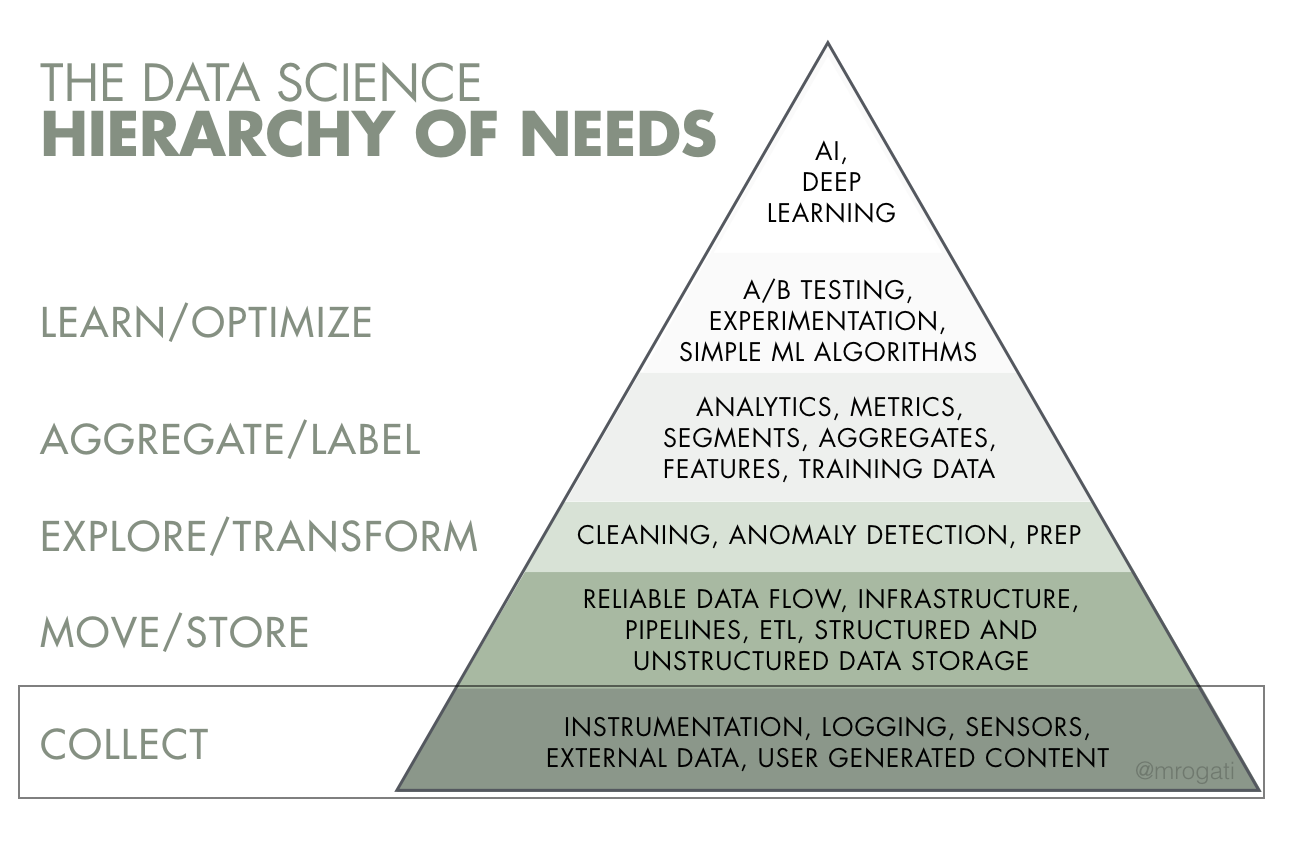
\includegraphics[width=14cm,height=12cm,keepaspectratio]{../media/crawler/data_hierarchy.png}
  \caption{\underline{Source}: Monica Rogati's "The AI hierarchy of Needs"}
  \label{fig:datahierarchy}
\end{figure}

Implementing a web crawler can be seen as a fancy project and its complexity can easily be overlooked.
Given the apparent simplicity of basic crawling algorithm. It posses numerous challenges. First of all,
crawling the whole web is simply unrealistic even for the world's most advanced crawlers. Considering the
current scale of web and while its still evolving, it is important to think thoroughly about
characteristics of a crawler, because this brings control in the hands of developers, it enriches the
value of problem they are trying to solve, it gives them a choice to either seek broad coverage over fresh
content or maintain a balance between the two. Even a small scale version of a crawler can be built to
be sophisticated and scalable. Moreover, building a crawler sets a playground to address problems such
as concurrency, throughput, and load balancing. It is a program quite different from traditional,
client-server paradigm that can fanout from single source file to modular, independent services that interact with each other through endpoints. 
\\
\\
When discussing a system like crawler, people often critic saying that
\\
\\
``Stop worrying about scale. You're not Google/Amazon. Just use a relational database.''
\\
\\
Well, that is true; building for scale without enough evidence from the metrics such as logging, locks you into an inflexible design. It is also a form
of premature optimization. Along the same lines, there is also an urge felt to overengineer and loose
focus on simplicity. Engineers loves to solve puzzles and challenge of building complex software. Overengineering is basically building a solution that is much more complex than is really necessary. This occurs when developer at a job tries to predict every possible use case and every edge case, eventually losing focus on the most common use cases.  
\\
\\
However, the author of this thesis believes that it important to survey different technologies as each have
their own strengths and weaknesses and choose the right tool for the job. The inclusion of message broker, docker, and AWS services to build the crawler are introduced with a mindset of promoting good design which will allow one to add more details and features later on. The design begins with a reasonable level of abstraction and with multiple iterations will gives better results.

%%% Local Variables:
%%% mode: latex
%%% TeX-master: "report"
%%% End:

